% =====================================================================
% JAMIA 2027 -- Research and Applications
%
% Journal of the American Medical Informatics Association (Oxford UP).
% Submission constraints encoded by this template:
%   * Main text  : 4,000 words maximum (Background and Significance
%                  through Conclusion; excludes abstract, references,
%                  tables, and figure legends)
%   * Abstract   : structured, 250 words maximum, with the headings
%                  Objective / Materials and Methods / Results /
%                  Discussion / Conclusion
%   * Tables     : 4 maximum        * Figures: 6 maximum
%   * References : unlimited, numbered in order of first appearance
%
% This file deliberately uses the stock `article' class so that it
% compiles in any TeX distribution. To typeset with Oxford's official
% class instead, install oup-authoring-template and replace the
% \documentclass line below with:
%   \documentclass[unnumsec,webpdf,contemporary,large]{oup-authoring-template}
% then delete the geometry/titlesec/abstract blocks, which that class
% supplies itself.
% =====================================================================
\documentclass[11pt,a4paper]{article}

\usepackage[T1]{fontenc}
\usepackage[utf8]{inputenc}
\usepackage{amsmath}
\usepackage{graphicx}
\usepackage{booktabs}
\usepackage{tabularx}
\usepackage{array}
\usepackage{makecell}
\usepackage{multirow}
\usepackage{xcolor}
\usepackage[margin=1in]{geometry}
\usepackage{titlesec}
\usepackage{authblk}

% JAMIA uses numbered citations set as superscripts, ordered by first
% appearance and placed after punctuation.
\usepackage[numbers,super,sort&compress]{natbib}

% Continuous line numbering and double spacing per JAMIA submission
% requirements ("all submissions should be double-spaced"). Line numbers
% assist peer review and are standard for the review copy.
\usepackage{lineno}\linenumbers
\usepackage{setspace}\doublespacing

\usepackage[colorlinks=true,allcolors=black]{hyperref}

% --------------------------------------------------------------
% DRAFT-ONLY ANNOTATIONS
% One switch controls every draft annotation in the manuscript: the
% pre-submission task list on the title page and all inline [TODO]
% markers. Flip it to \showtasksfalse to produce a clean submission
% PDF -- nothing else needs editing.
% --------------------------------------------------------------
\newif\ifshowtasks
\showtasksfalse         % <-- set to \showtaskstrue while drafting

\newcommand{\TODO}[1]{\ifshowtasks\textcolor{red}{\textbf{[TODO: #1]}}\fi}

% JAMIA sets primary headings in full capitals.
\titleformat{\section}{\normalfont\large\bfseries}{\thesection.}{0.6em}{\MakeUppercase}
\titleformat{\subsection}{\normalfont\normalsize\bfseries}{\thesubsection.}{0.6em}{}

\renewcommand{\abstractname}{ABSTRACT}

\begin{document}

% ---------------------------------------------------------------------
% Title and authors
% ---------------------------------------------------------------------
\title{\bfseries Automated, Component-Level Assessment of a National
Inpatient Diabetes Guideline: Adherence and Its Association with
Hospitalization Complications Across Six Hospitals}

% TODO(pre-submission): confirm degrees with each co-author before
% submission. JAMIA requires the degree of every co-author on the title
% page. Shahar Oded is BSc pre-graduation; update to MSc after the
% degree is conferred (expected late 2026).
\author[1,$\ast$]{Shahar Oded,~BSc\thanks{\textbf{Corresponding author.}
Shahar Oded, Medical Informatics Research Center, Ben-Gurion University of
the Negev.
Postal address: Honi Hameagel~7, Tel Aviv, Israel, 6266307.
Telephone: +972-54-484-5432.
Email: \href{mailto:shahar6771@gmail.com}{shahar6771@gmail.com}.}}
\author[1]{Yuval Shahar,~MD,~PhD}
\author[1]{Erez Shalom,~PhD}
\author[2,3]{Amir Bashkin,~MD}
\author[4,5]{Leonard Saiegh,~MD}
\author[6]{Dror Cantrell,~\textcolor{red}{[degree TBC]}}
\author[7]{Irit Wirsansky,~\textcolor{red}{[degree TBC]}}
\author[2,8]{Muhamad Badarne,~\textcolor{red}{[degree TBC]}}
\author[9]{Irena Barash,~\textcolor{red}{[degree TBC]}}
\author[10,11]{Avivit Cahn,~MD}
\author[4,7]{Irit Hochberg,~MD,~PhD}

\affil[1]{Medical Informatics Research Center, Ben-Gurion University of the
Negev, Beer Sheva, Israel}
\affil[2]{Azrieli Faculty of Medicine, Bar-Ilan University, Safed, Israel}
\affil[3]{Endocrinology and Diabetes Unit, Galilee Medical Center,
Nahariya, Israel}
\affil[4]{Bruce Rappaport Faculty of Medicine, Technion--Israel Institute
of Technology, Haifa, Israel}
\affil[5]{Endocrinology Institute, Bnai Zion Medical Center, Haifa, Israel}
\affil[6]{Internal Medicine Department C, Shamir Medical Center,
Beer Yaakov, Israel}
\affil[7]{Endocrinology Unit, Hillel Yaffe Medical Center, Hadera, Israel}
\affil[8]{Endocrinology and Diabetes Service, Tzafon Medical Center,
Ramat Poriya, Israel}
\affil[9]{Internal Medicine Department C, Barzilai Medical Center,
Ashkelon, Israel}
\affil[10]{Internal Medicine Department A, Hadassah Ein Kerem, Jerusalem,
Israel}
\affil[11]{Faculty of Medicine, Hadassah Hebrew University Hospital,
Jerusalem, Israel}

\date{}
\maketitle

% JAMIA title page must state the exact body word count, excluding title
% page, abstract, tables, figures, references, and acknowledgments.
% Recount before submission with:
%   texcount -inc -brief -sum=1,0,0,0 background.tex methods.tex \
%            results.tex discussion.tex conclusion.tex
{\centering\noindent\textbf{Word count (main text):} 3{,}969\par}
\vspace{0.8em}

% ---------------------------------------------------------------------
% Draft-only task list (suppressed by \showtasksfalse; not part of the
% manuscript and not counted toward the 4,000-word limit).
% Guarded, so the manuscript still compiles wherever this draft-only
% file is absent -- e.g. a submission upload that omits it.
% ---------------------------------------------------------------------
\IfFileExists{tasks.tex}{% =====================================================================
% DRAFT-ONLY: pre-submission task list.
%
% Rendered only while \showtaskstrue is set in main.tex. It carries no
% manuscript content and is excluded from the 4,000-word count.
% Flipping the switch to \showtasksfalse removes this box and every
% inline [TODO] marker at once.
% =====================================================================
\ifshowtasks
\begin{center}
\fcolorbox{red}{red!4}{%
\begin{minipage}{0.94\textwidth}
\vspace{2pt}
\textcolor{red}{\textbf{DRAFT --- OPEN TASKS BEFORE SUBMISSION}}
\vspace{4pt}
\hrule
\vspace{6pt}
\footnotesize
\begin{enumerate}\setlength{\itemsep}{5pt}\setlength{\parskip}{0pt}

\item \textbf{Funding statement.} Name the funding body and grant number,
or state that the work received no specific grant. Oxford registers
funders through the Crossref Funding Data Registry, so the funder name
must match its canonical form there. \emph{(Section: Funding.)}

\item \textbf{Export the curated concept indices from the closed
environment.} The manuscript now states that the indices are provided as
supplementary material (Methods, Appendix~S1, and the Data Availability
statement all say so). That claim is not yet true --- the files must be
exported from the hospital VM and attached before submission, or all
three statements must be walked back.

\end{enumerate}
\vspace{4pt}
\end{minipage}}
\end{center}
\vspace{6pt}
\fi
}{}

% ---------------------------------------------------------------------
% Structured abstract (250 words max)
% ---------------------------------------------------------------------
\begin{abstract}
\noindent
\textbf{Objective:}
To measure adherence to a national inpatient hyperglycemia guideline at the
level of its individual recommendations across a hospital network, to
determine whether it changed after the guideline was issued, and to identify
which recommendations track subsequent outcomes.

\noindent
\textbf{Materials and Methods:}
Retrospective multicenter study of 48,354 admissions among 29,577 adults
with diabetes or inpatient hyperglycemia at six Israeli general hospitals,
August 2022 to December 2025. Each of 14 recommendations was formalized as a
quality-assessment temporal pattern over knowledge-based temporal
abstractions of the record, scored wherever it applied. Pre--post adherence was compared by
Welch $t$-test with false discovery rate correction. Associations with 10
complications were estimated by bias-reduced logistic regression over 24-,
48-, and 72-hour windows, and by inverse probability of
treatment weighting contrasting above- with at-or-below-median adherence.

\noindent
\textbf{Results:}
Adherence ranged from near-universal admission and medication-management
actions to substantial gaps in insulin management (means, 0.15--0.28). Overall adherence rose modestly after issue (0.682 to 0.703,
$P<.001$), with marked inter-hospital heterogeneity. After weighting,
above-median adherence carried 44\% lower odds of 30-day mortality (odds
ratio [OR], 0.557; 95\% CI, 0.514--0.603), 82\% lower odds of hyperglycemia
(OR, 0.175) and 52\% lower odds of severe hyperglycemia (OR, 0.485), against
20\% higher odds of hypoglycemia (OR, 1.204).

\noindent
\textbf{Discussion:}
The least-implemented recommendations were largely those whose adherence
tracked outcomes: repeated insulin decisions spread across a stay, rather
than discrete actions on admission.

\noindent
\textbf{Conclusion:}
Guideline adherence can be assessed automatically and per-recommendation at
national scale, identifying where fuller implementation would most plausibly
matter.
\end{abstract}

\vspace{0.5em}
\noindent
\textbf{Keywords:} inpatient diabetes; guideline adherence; temporal
abstraction; electronic health records; propensity score


% ---------------------------------------------------------------------
% Main text (4,000 words max)
% ---------------------------------------------------------------------
\section{Background and Significance}
\label{sec:background}

Diabetes mellitus affects approximately 537 million adults worldwide, a figure
projected to reach 783 million by 2045 \citep{idf-atlas-10th-edition-2021}. In
Israel, the national registry documents a steadily growing patient population
and a corresponding burden on the health system
\citep{israel-national-center-disease-control-diabetes-registry-report-2012-2022,
summary-cost-diabetes-israel-2018}, concentrated in hospital care:
approximately 40\% of patients admitted to Israeli general hospitals have
diabetes \citep{hochberg2023inpatient}.

In hospital the clinically relevant object is not the diagnosis but the
glycemic state during the admission. Hyperglycemia arising in hospital is
associated with infection, delayed healing, metabolic decompensation and
increased mortality, and occurs in patients with and without documented
diabetes. Its counterpart, hypoglycemia, is acute, harmful, and largely
iatrogenic---a consequence of the insulin used to correct the first problem.
Inpatient glycemic management is therefore a balancing act shaped less by any
single decision than by how monitoring, medication management and insulin
dosing are carried out repeatedly across a stay. That makes the treatment
process itself, not only the patient's state, worth measuring.

In September 2023 the Israel Endocrine Society, the Israel Diabetes Association
and the National Diabetes Council issued a national position paper on inpatient
diabetes care \citep{hochberg2023inpatient}, specifying how often glucose
should be measured, how oral antidiabetic agents should be handled on
admission, when basal and correction insulin should be given, and how to
respond to glycemic episodes. Recommendations of this kind are checkable in
principle because they are procedural, temporal and conditional: an action is
expected, within some window or at some frequency, when a triggering situation
holds. Establishing whether they were followed is harder, having conventionally
required chart review, which does not scale past modest single-institution
samples---too small to separate one ward's practice from the effect of a
guideline, and far too small to observe how practice shifts when a guideline is
introduced nationally.

Informatics supplies the machinery to do this automatically. Knowledge-based
temporal abstraction and the Temporal Mediator \citep{shahar1997framework} turn
time-stamped clinical data into named interval concepts; Asbru
\citep{shahar1997asbru, shahar1998asgaard} expresses a guideline's procedural
content as a hierarchy of execution plans; and Picard
\citep{shalom2016architecture} combines the two to generate real-time
recommendations and adherence reports. Deployed in MobiGuide
\citep{peleg2022mobiguide}, it raised clinicians' guideline compliance from
41\% to 93\%---direct evidence that adherence is malleable, and therefore worth
measuring. Retrospective assessment required a third body of knowledge:
\emph{quality-assessment} knowledge \citep{ben2024supporting} re-expresses that
procedural content declaratively, as the temporal pattern correct execution
would have left in the record, with a membership function grading partial
compliance rather than a binary verdict. Such systems have been validated
against simulated scenarios \citep{shalom2015multiple} and applied
institutionally to long-term management at a geriatric hospital
\citep{shalom2024implementation}.

This study adopts that formulation of adherence but not the systems that
introduced it, and departs from them in three respects. In
\emph{representation}, procedural and declarative knowledge are encoded in a
single schema evaluated by one engine, and the resulting knowledge base is
itself a transferable contribution. In \emph{scale}, adherence is measured
across six hospitals spanning a national implementation rather than within one
institution. In \emph{purpose}, prior work evaluates care \emph{against} the
guideline, which serves as the reference standard; here each recommendation is
treated as a hypothesis to be tested against what subsequently happened to the
patient. Adherence thus becomes an explanatory variable: the question is not
whether the guideline was applied correctly, but which of its recommendations
demonstrably matter.

\section{Objective}
\label{sec:objective}

We set out to determine, across a national hospital network spanning the
introduction of an inpatient hyperglycemia guideline, how completely each of
its individual recommendations was implemented and whether that changed after
the guideline was issued; whether adherence is associated with subsequent
complications once measured patient characteristics are accounted for; and
which individual recommendations carry that association.

\section{Materials and Methods}
\label{sec:methods}

\subsection{Study design and data source}

We conducted a retrospective multicenter study using electronic health record
data from six Israeli general hospitals, drawn from Kineret
\citep{rappoport2025kineret}, the data warehouse of Israel's largest hospital
network, represented in the Observational Medical Outcomes Partnership (OMOP)
common data model. The assessed recommendations are those of the national
position paper on the treatment of diabetes in hospitalization in a general
hospital \citep{hochberg2023inpatient}, issued in September 2023. The
pre-intervention period ends immediately before publication (August 2022--July
2023) and the post-intervention period begins a year after it (August
2024--December 2025), the intervening months being excluded to allow for
staggered adoption.

Kineret was not mapped to an international coding system at the time of this
work, so a dataset-specific concept index---a many-to-one mapping from local
codes onto the concepts named in the knowledge base---was curated first. That
index is what makes the remainder of the pipeline dataset-agnostic: once it
exists, the same knowledge base and engine run unchanged on any source within
the same clinical scope. The curated indices are provided as supplementary
material, and the curation procedure is described in Supplementary
Appendix~S1.

\subsection{Cohort definition}
\label{sec:cohort-definition}

An admission was eligible if it was an inpatient visit of 48 hours to 14 days
in a patient aged at least 18 years, with evidence of a genuine overnight stay,
no death within 48 hours of admission, no admission to an excluded department,
and at least one criterion for diabetes or hyperglycemia. Excluding pediatric
and obstetric departments also removes pregnancy-related admissions. Diabetes or
hyperglycemia was established by at least one of three non-mutually-exclusive
criteria: a documented diabetes
diagnosis from a manually curated list of concept identifiers; recurrent
hyperglycemia, two glucose measurements $\geq$180 mg/dL separated by 2 to 24
hours; or extreme hyperglycemia, any glucose measurement $\geq$250 mg/dL.
Hypoglycemia was deliberately not an entry criterion: the cohort is defined by
hyperglycemic burden, and hypoglycemia is treated throughout as an outcome
rather than as a route into the study population. Full eligibility rules are
given in Supplementary Appendix~S1.

\subsection{Abstraction input}

The \emph{temporal input} is a long-format table in which each row records one
time-stamped clinical fact, with structural tokens inserted to make the
admission timeline explicit---notably recurring \textsc{meal} tokens, assumed
to fall at fixed daily times because meal times are not recorded in the source
data. The \emph{context input} holds one row per admission of baseline
characteristics from the first 48 hours, from which a modified Charlson
comorbidity index (CCI) was computed (Supplementary Appendix~S1).

\subsection{Guideline adherence assessment}

Adherence was assessed by knowledge-based temporal abstraction
\citep{shahar1997framework}, which converts time-stamped clinical data into
named interval concepts and then detects, over those intervals, the temporal
pattern that correct execution of each recommendation would have left in the
record \citep{ben2024supporting}. Abstraction and assessment are performed in a
single pass by our reimplementation of the Temporal Mediator
\citep{mediator-github}. All domain knowledge is declared externally as XML
units validated against a shared schema, so that the clinical semantics and the
guideline requirements are stated once, outside the analysis code.

Each recommendation is formalized as a quality-assessment temporal pattern: an
\emph{anchor} identifying the clinical situation in which it applies, an
\emph{action} that satisfies it, a constraint type, and a membership function
grading partial compliance. Applicability is enforced by context---an anchor
falling outside the context in which the recommendation holds generates no
obligation and is not scored---so that an insulin dose after a meal is required
only where glucose is elevated. Recurring recommendations such as routine
glucose monitoring are instead evaluated by counting qualifying events within
fixed-length windows.

Compliance is graded rather than binary. Each constraint carries a trapezoidal
membership function mapping observed timing, frequency, or value to $[0,1]$: if
correction insulin is expected within 4 hours of a hyperglycemic reading and
considered missed after 12, insulin given at 8 hours scores 0.5 rather than
counting as an outright failure. Three constraint types are
used---\emph{time}, \emph{value}, and \emph{cyclic}---corresponding to the
compliance aspects reported below. An unanswered anchor
scores 0 where the recommendation requires an action, and 1 where it requires
one to be withheld, since there the absence of a response is itself compliant;
a recommendation that never became applicable yields no output rather than a
zero, so inapplicable recommendations do not depress the score.

Fourteen recommendations were formalized by the first author under the guidance
of two co-authors specializing in temporal reasoning and in diabetes care, who
reviewed them for clinical fidelity against the source position paper. Scoring
is retrospective and offline: the procedure issues no recommendation and
returns nothing to the treating team. Thresholds and the full pattern
definitions are given in Supplementary Appendices~S1 and~S3.

\subsection{Outcome definitions}

Ten complications were evaluated: 30-day mortality, hyperglycemia, severe
hyperglycemia, hypoglycemia, severe hypoglycemia, hyperosmolality,
ketoacidosis, infection, inpatient acute kidney injury, and inpatient
myocardial infarction. All ten are emitted as abstractions by the same engine,
so that outcome ascertainment and adherence assessment draw on a single
explicit knowledge base. Thirty-day mortality was taken from linked death
records, defined as death between 14 days before and 30 days after the recorded
discharge datetime, the backward tolerance capturing in-hospital deaths whose
death record precedes the discharge timestamp. Operational definitions are
given in Supplementary Appendix~S2.

\subsection{Statistical analysis}

The admission is the unit of analysis. Compliance scores were collapsed
successively over compliance aspects, calendar days, and finally patterns with
equal weight, so that neither frequently-evaluated patterns nor
frequently-evaluated days dominate the resulting per-admission score
(Supplementary Appendix~S1).

Adherence was compared between periods by Welch's unequal-variance $t$-test,
each admission attributed by its admission date. Confidence intervals are
unadjusted Welch $t$-intervals, and $P$ values were adjusted across
component-level comparisons by the Benjamini--Hochberg false discovery rate
(FDR) procedure \citep{benjamini1995controlling}. Monthly means carry 95\% CIs
from the within-month standard error, and the temporal trend is an ordinary
least-squares fit to those means.

Whole-admission adherence was compared between admissions ending in death
within 30 days and those not, and the graded relationship tested by logistic
regression on the continuous score, reported as the odds ratio (OR) per
0.1-point increase, then adjusted for age, sex, modified CCI, and hospital with
standard errors clustered on patient identity. Both are descriptive, since
whole-admission adherence does not strictly precede the outcome.

To identify which individual recommendations were associated with each
complication, one model was fitted per complication at cutoffs of 24, 48, and
72 hours. Each row is an admission--complication pair, labelled positive if the
complication first occurred at or after the cutoff and negative if it never
occurred; admissions in which it occurred \emph{before} the cutoff were
excluded, since a pre-existing condition cannot be attributed to subsequent
in-stay care, and adherence and covariates were computed only up to the cutoff.
Models were fitted by bias-reduced (Firth penalized-likelihood) logistic
regression \citep{firth1993bias}, unpenalized maximum likelihood having failed
to converge under separation for most complications. Correlated predictors were
pruned and the remainder standardized, and a predictor was considered robust
only if it remained significant with consistent direction across all three
windows. To avoid mechanical circularity, routine glucose monitoring was
excluded from the glycemic models, since glucose measurement is itself the
mechanism by which those events are detected.

Because these models estimate conditional predictive associations rather than
treatment effects, overall adherence and the recurrent components were
re-evaluated by inverse probability of treatment weighting, with adherence
dichotomized at the median of each outcome's eligible population. The binary
exposure is intrinsic to the design rather than a simplification, since the
propensity score \citep{rosenbaum1983central} and the standardized mean
differences (SMDs) used to verify balance \citep{austin2009balance} are
two-group constructs undefined for a continuous exposure; retaining continuous
adherence in the regressions above therefore makes the two designs
complementary. Propensity scores were estimated by bias-reduced logistic
regression, converted to stabilized weights and trimmed at the 1st and 99th
percentiles. Balance was assessed by the maximum post-weighting SMD, with
$<$0.10 required for an estimate to be interpretable; pairs failing this are
reported as non-estimable. Confidence intervals are unadjusted throughout, so an
interval excluding the null may accompany a nonsignificant adjusted $P$ value.
Analyses used Python 3.13 (Supplementary Appendix~S1).

\section{Results}
\label{sec:results}

\subsection{Study cohort}

The cohort comprised 48,354 admissions among 29,577 unique adult patients
across six Israeli general hospitals, with center-specific sample sizes ranging
from 4,478 to 11,024 admissions (Table~\ref{tab:cohort}). Only 21.5\% of
admissions meeting a hyperglycemia criterion carried a documented diabetes
diagnosis, indicating that a substantial proportion of the cohort represented
clinically significant inpatient hyperglycemia without a recorded diagnosis.

\subsection{Adherence and its change following national implementation}
\label{sec:adherence-results}

Adherence varied sharply across recommendations, and the split followed the
kind of action required rather than its clinical weight
(Table~\ref{tab:adherence}). Single discrete actions on admission were
near-universal: SGLT2 discontinuation was complete (1.00) and creatinine
measurement almost so (0.98). Recommendations calling for repeated insulin
decisions across the stay were not: insulin following hyperglycemia scored 0.15, the
two routine basal dosing components 0.21 and 0.23, and bolus reduction after
hypoglycemia 0.28---all with a median of zero, meaning the expected action
was absent altogether in most eligible admissions. Monitoring and admission
medication management fell between these extremes (0.54--0.88). Adherence was
largely independent of whether diabetes had been formally documented (0.669 vs
0.661 among admissions with hyperglycemia in the first 48 hours), a difference
reaching significance only by virtue of the sample size.

Overall adherence rose from 0.682 before the guideline to 0.703 after
($P<.001$; Figure~\ref{fig:adherence-trend}), with monthly scores trending
upward across the period. The absolute change is small, and its significance
reflects the number of admissions rather than the size of the shift.
Component-level changes were uneven (Table~\ref{tab:adherence}). Glucose
monitoring improved most---on admission from 0.78 to 0.93---and discontinuation
of high-hypoglycemia-risk antidiabetic agents on admission rose from 0.62 to
0.75. Gains in the insulin-management components were significant but marginal
($+$0.01 to $+$0.03), leaving them close to their already low baselines, while
dose reduction after hypoglycemia did not change and SGLT2 discontinuation was
already complete in both periods. Center-level trajectories ranged from
improvement through no measurable change to modest decreases, so the pooled
increase conceals substantial inter-hospital heterogeneity.

\subsection{Adherence and clinical outcomes}

Higher adherence was associated with lower 30-day mortality
(Figure~\ref{fig:adherence-mortality}). Survivors had a higher mean adherence
score than those who died (0.693 vs 0.652, $P<.001$), and mortality fell across
adherence strata from 11\% to roughly 3\%. On the continuous score, each
0.1-point increase carried 16.8\% lower odds of death (OR, 0.832; 95\% CI,
0.811--0.853), so the association is graded rather than threshold-like, and
adjusting for age, sex, comorbidity burden and hospital left it intact
(adjusted OR, 0.757; 95\% CI, 0.727--0.788, per 1-SD increase). Adherence to the insulin-management
recommendations showed negligible correlation with subsequent hypoglycemic
burden, for both hypoglycemia ($r=0.052$) and severe hypoglycemia ($r=0.056$;
$n=40{,}719$).

\subsection{Outcome-associated recommendations}

Between 9 and 34 predictors were retained per outcome, but the number
surviving all three window definitions ranged from none to 32, tracking event
frequency: mortality yielded the most robust predictors and the rarer
complications few or none (Supplementary Table~S2). For mortality, the model
recovered well-established clinical predictors---age, red cell distribution
width, body mass index (BMI), dementia, cardiovascular comorbidity---which
gives the approach face validity, and several adherence components ranked among
the strongest retained predictors (Figure~\ref{fig:death-importance}). Across
all outcome models (Figure~\ref{fig:recurring-guidelines}), insulin following
hyperglycemia and admission glucose monitoring recurred most broadly, while
basal-dose components appeared in fewer, more outcome-specific models.
Direction was not uniform---the same component could carry opposite signs for
different endpoints.

\subsection{Propensity-weighted evaluation}

The overall-adherence analyses achieved satisfactory covariate balance (maximum
post-weighting SMD $<$0.08). Relative to the low-adherence group, above-median
adherence carried 44\% lower odds of 30-day mortality (OR, 0.557; 95\% CI,
0.514--0.603), 82\% lower odds of hyperglycemia (OR, 0.175) and 52\% lower odds
of severe hyperglycemia (OR, 0.485), all adjusted $P<.001$, against 20\% higher
odds of hypoglycemia (OR, 1.204; 95\% CI, 1.090--1.331;
Table~\ref{tab:iptw-overall}). Nothing survived correction for the remaining
five outcomes. The asymmetry between those two directions is the substantive
result: the reduction in hyperglycemic burden is roughly ninefold larger on the
log-odds scale than the accompanying increase in hypoglycemia, and the increase
in \emph{severe} hypoglycemia did not reach significance (OR, 1.129; adjusted
$P=.096$).

Only a subset of the recurrent component-level predictors remained significant
after weighting, indicating that several predictive associations were largely
explained by differences in baseline patient characteristics. A further six
significant associations were set aside because weighting failed to achieve
acceptable balance (maximum SMD, 0.90--2.46). All six concerned BMI or
creatinine measurement on admission, for which adherence is near-universal, so
that dichotomizing at the median produces groups too dissimilar to balance;
those coefficients were numerically degenerate and are reported as
non-estimable.

Eight associations were both significant and adequately balanced
(Table~\ref{tab:iptw-patterns}). Above-median adherence to routine basal
insulin dosing, routine glucose monitoring and insulin administration following
hyperglycemia each remained associated with lower 30-day mortality. For
glycemic outcomes, insulin following hyperglycemia (78\% lower odds; OR, 0.220)
and routine basal insulin dosing (60\% lower odds; OR, 0.402) were associated
with substantially lower odds of subsequent severe hyperglycemia, while insulin
following hyperglycemia also carried 28\% higher odds of hypoglycemia (OR,
1.283)---the same trade-off seen at the level of overall adherence. Adherence to glucose monitoring on
admission was associated with a higher recorded incidence of hyperglycemia and
severe hyperglycemia; since these outcomes are ascertained from glucose
measurements, more frequent early measurement mechanically increases the chance
of recording an event, so both associations likely reflect ascertainment rather
than harm.

These are the same components that showed the largest implementation gaps:
insulin following hyperglycemia (mean adherence, 0.15) and routine basal
insulin dosing (0.21--0.23) are simultaneously the least-implemented
recommendations assessed and, after weighting, among those most strongly
associated with mortality and with severe hyperglycemia.

% =====================================================================
% Table 1
% =====================================================================
\begin{table}[t]
\centering
\caption{Characteristics of the multicenter study cohort.}
\label{tab:cohort}
\small
\begin{tabularx}{\textwidth}{
>{\raggedright\arraybackslash}X
>{\raggedleft\arraybackslash}p{0.34\textwidth}
}
\toprule
Characteristic & Value \\
\midrule
Hospitals & 6 \\
Admissions & 48,354 \\
Unique patients & 29,577 \\
Age, mean (median), y & 71.9 (73.3) \\
Male sex & 54.3\% \\
Length of stay, median, d & 5.55 \\
30-day mortality & 9.58\% \\
\midrule
Documented diabetes diagnosis & 35.3\% \\
Recurrent hyperglycemia & 74.7\% \\
Extreme glucose ($\geq$250 mg/dL) & 60.2\% \\
Hyperglycemia among admissions with diabetes & 50.3\% \\
Diabetes diagnosis among admissions with hyperglycemia & 21.5\% \\
\midrule
Pre-intervention cohort &
\makecell[r]{21,605 admissions\\17,002 patients} \\
Post-intervention cohort &
\makecell[r]{16,182 admissions\\11,201 patients} \\
\bottomrule
\end{tabularx}
\end{table}

% =====================================================================
% Table 2 -- merged overall adherence + pre/post change
% =====================================================================
\begin{table}[t]
\centering
\caption{Adherence to each assessed inpatient diabetes guideline
recommendation over the whole study period, and its change following
national implementation. Scores range from 0 (nonadherence) to 1 (complete
adherence). $\Delta$ is the absolute difference in mean adherence between the
post- and pre-intervention periods, with unadjusted 95\% CIs; $P$ values were
adjusted across component-level comparisons using the Benjamini--Hochberg
false discovery rate procedure.}
\label{tab:adherence}
\small
\setlength{\tabcolsep}{4pt}
\begin{tabularx}{\textwidth}{
>{\raggedright\arraybackslash}X
rrrrlr
}
\toprule
Recommendation & Mean & Median & Before & After & $\Delta$ (95\% CI) & $P$ \\
\midrule
Admission glucose monitoring
  & 0.85 & 1.00 & 0.78 & 0.93 & $+$0.15 (0.145 to 0.154) & $<.001$ \\
Routine glucose monitoring
  & 0.88 & 0.98 & 0.83 & 0.94 & $+$0.11 (0.105 to 0.113) & $<.001$ \\
Glucose monitoring during corticosteroid therapy
  & 0.54 & 0.50 & 0.51 & 0.58 & $+$0.07 (0.062 to 0.087) & $<.001$ \\
BMI measurement on admission
  & 0.87 & 1.00 & 0.86 & 0.89 & $+$0.03 (0.015 to 0.029) & $<.001$ \\
Creatinine measurement on admission
  & 0.98 & 1.00 & 0.98 & 0.99 & $+$0.01 (0.008 to 0.014) & $<.001$ \\
Antidiabetic discontinuation on admission
  & 0.66 & 0.86 & 0.62 & 0.75 & $+$0.13 (0.075 to 0.192) & $<.001$ \\
SGLT2 discontinuation on admission
  & 1.00 & 1.00 & 1.00 & 1.00 & 0.00 (--) & -- \\
Basal insulin continuation on admission
  & 0.66 & 1.00 & 0.63 & 0.67 & $+$0.04 (0.002 to 0.089) & .054 \\
Insulin administration after hyperglycemia
  & 0.15 & 0.00 & 0.14 & 0.15 & $+$0.01 (0.009 to 0.020) & $<.001$ \\
Antidiabetic discontinuation after hypoglycemia
  & 0.89 & 1.00 & 0.91 & 0.89 & $-$0.02 ($-$0.197 to 0.158) & .818 \\
Basal dose reduction after hypoglycemia
  & 0.87 & 1.00 & 0.87 & 0.88 & $+$0.01 ($-$0.015 to 0.034) & .497 \\
Bolus dose reduction after hypoglycemia
  & 0.28 & 0.00 & 0.33 & 0.26 & $-$0.07 ($-$0.158 to 0.029) & .210 \\
Routine basal dosage (frequency)
  & 0.23 & 0.00 & 0.21 & 0.24 & $+$0.03 (0.027 to 0.043) & $<.001$ \\
Routine basal dosage (dose)
  & 0.21 & 0.00 & 0.19 & 0.22 & $+$0.03 (0.021 to 0.036) & $<.001$ \\
\bottomrule
\end{tabularx}
\end{table}

% =====================================================================
% Table 3 -- IPTW, overall adherence
% =====================================================================
\begin{table}[t]
\centering
\caption{Inverse probability of treatment weighting analysis of overall
guideline adherence. Adherence was dichotomized at the median of each
outcome's eligible population, so $\beta$ is the log-odds ratio comparing the
above-median with the at-or-below-median group and OR $=\exp(\beta)$.
Confidence intervals are unadjusted; $P$ values were adjusted across outcomes
using the Benjamini--Hochberg false discovery rate procedure. Balance was
assessed by the maximum standardized mean difference (SMD) after weighting.
AKI, acute kidney injury; MI, myocardial infarction.}
\label{tab:iptw-overall}
\small
\setlength{\tabcolsep}{4pt}
\begin{tabular}{lrrlrr}
\toprule
Outcome & $\beta$ & OR & 95\% CI (OR) & Max SMD & $P$ \\
\midrule
Hyperglycemia        & $-1.742$ & 0.175 & 0.154 to 0.199 & 0.019 & $<.001$ \\
Severe hyperglycemia & $-0.724$ & 0.485 & 0.450 to 0.523 & 0.012 & $<.001$ \\
30-day mortality     & $-0.586$ & 0.557 & 0.514 to 0.603 & 0.020 & $<.001$ \\
Hypoglycemia         & $0.186$  & 1.204 & 1.090 to 1.331 & 0.034 & $<.001$ \\
Severe hypoglycemia  & $0.121$  & 1.129 & 1.001 to 1.274 & 0.030 & .096 \\
Hyperosmolarity      & $0.106$  & 1.112 & 0.652 to 1.896 & 0.020 & .800 \\
Ketoacidosis         & $0.116$  & 1.123 & 0.561 to 2.246 & 0.021 & .800 \\
Inpatient MI         & $0.055$  & 1.057 & 0.732 to 1.523 & 0.020 & .800 \\
Infection            & $-0.025$ & 0.975 & 0.809 to 1.175 & 0.020 & .800 \\
Inpatient AKI        & $0.018$  & 1.018 & 0.888 to 1.168 & 0.022 & .800 \\
\bottomrule
\end{tabular}
\end{table}

% =====================================================================
% Table 4 -- IPTW, individual recommendations
% =====================================================================
\begin{table}[t]
\centering
\caption{Inverse probability of treatment weighting analysis of individual
guideline recommendations. Rows are the component--outcome pairs that were
both statistically significant after false discovery rate correction and
adequately balanced after weighting (maximum standardized mean difference
$<$0.10). A further six significant associations, all concerning BMI or
creatinine measurement on admission, failed the balance criterion (maximum
standardized mean difference, 0.90--2.46) and are not reported.
$^{\dagger}$Likely to reflect ascertainment rather than harm: the outcome is
detected from glucose measurements, so more frequent early measurement
increases the opportunity to record an event.}
\label{tab:iptw-patterns}
\small
\setlength{\tabcolsep}{4pt}
\begin{tabular}{llrrlr}
\toprule
Outcome & Recommendation & $\beta$ & OR & 95\% CI (OR) & $P$ \\
\midrule
30-day mortality & Routine basal dosage
  & $-0.291$ & 0.748 & 0.691 to 0.809 & $<.001$ \\
30-day mortality & Routine glucose monitoring
  & $-0.139$ & 0.870 & 0.809 to 0.937 & $<.001$ \\
30-day mortality & Insulin after hyperglycemia
  & $-0.098$ & 0.907 & 0.842 to 0.977 & .011 \\
\midrule
Severe hyperglycemia & Insulin after hyperglycemia
  & $-1.514$ & 0.220 & 0.202 to 0.239 & $<.001$ \\
Severe hyperglycemia & Routine basal dosage
  & $-0.912$ & 0.402 & 0.372 to 0.434 & $<.001$ \\
Severe hyperglycemia & Admission glucose monitoring$^{\dagger}$
  & $0.752$ & 2.121 & 1.974 to 2.280 & $<.001$ \\
\midrule
Hyperglycemia & Admission glucose monitoring$^{\dagger}$
  & $0.980$ & 2.664 & 2.389 to 2.971 & $<.001$ \\
\midrule
Hypoglycemia & Insulin after hyperglycemia
  & $0.249$ & 1.283 & 1.163 to 1.416 & $<.001$ \\
\bottomrule
\end{tabular}
\end{table}

% =====================================================================
% Figures
% =====================================================================
\begin{figure}[t]
\centering
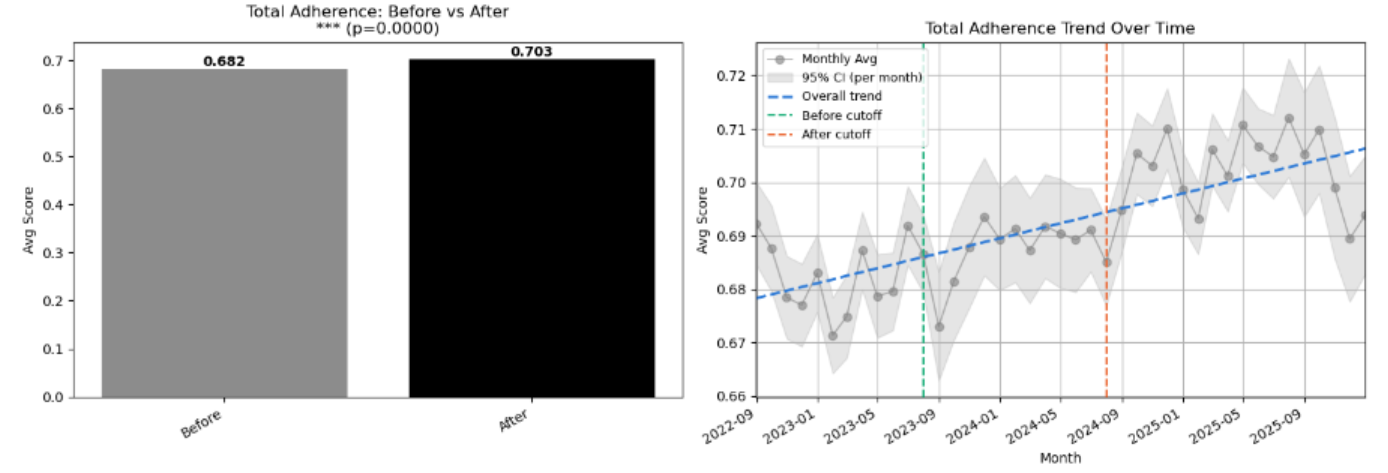
\includegraphics[width=\textwidth]{figures/adherence_trend.png}
\caption{Changes in overall guideline adherence across the study period.
\textbf{Left:} mean overall adherence during the predefined pre-intervention
(August 2022--July 2023) and post-intervention (August 2024--December 2025)
periods. \textbf{Right:} monthly mean overall adherence with 95\% CIs.
Vertical dotted lines delimit the transition period excluded from the primary
pre--post comparison; the dashed line indicates the overall temporal trend.}
\label{fig:adherence-trend}
\noindent\textit{Alt text:} Bar chart and monthly timeline plot illustrating
overall guideline adherence before and after September 2023.
\end{figure}

\begin{figure}[t]
\centering
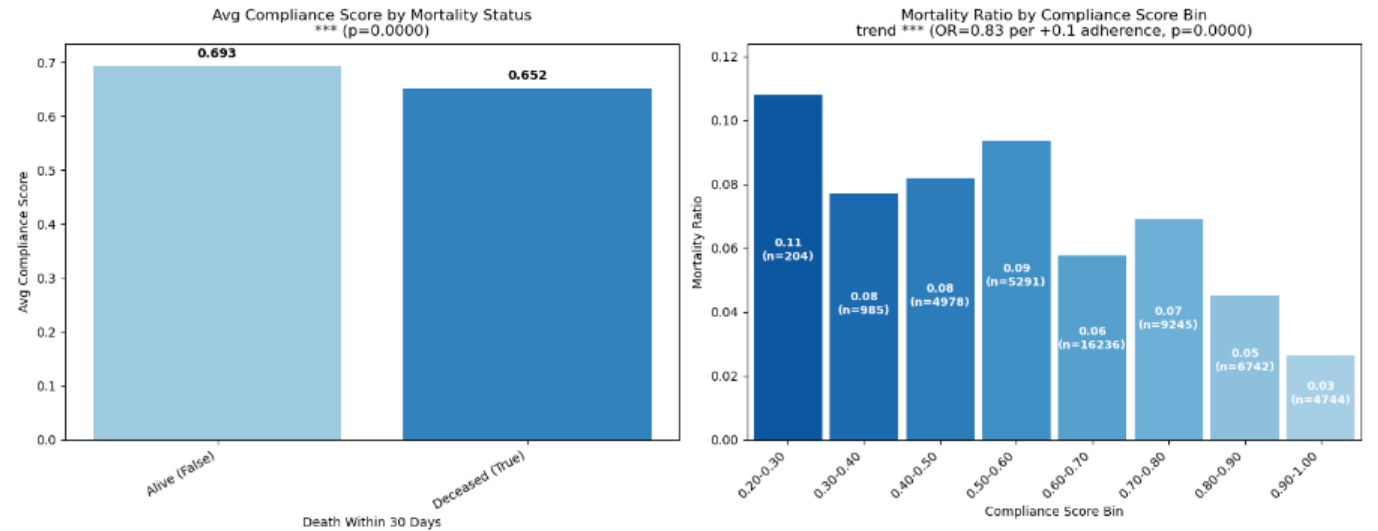
\includegraphics[width=\textwidth]{figures/adherence_mortality.png}
\caption{Association between overall guideline adherence and 30-day
mortality. \textbf{Left:} mean overall adherence among patients who survived
and those who died within 30 days. \textbf{Right:} observed 30-day mortality
across strata of overall adherence, with the number of admissions shown
within each bar; strata containing fewer than 30 admissions are not shown.
The trend statistic is from logistic regression on the continuous adherence
score, not on the binned values, and is expressed as the odds ratio per
0.1-point increase.}
\label{fig:adherence-mortality}
\noindent\textit{Alt text:} Bar charts displaying average guideline adherence
by 30-day mortality status and mortality rates across adherence deciles.
\end{figure}

\begin{figure}[t]
\centering
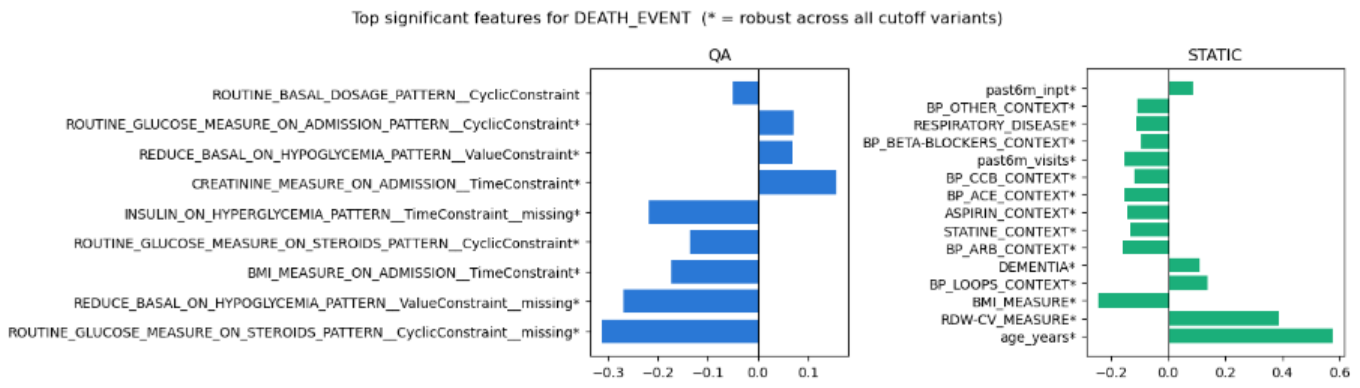
\includegraphics[width=\textwidth]{figures/death_feature_importance.png}
\caption{Retained feature profile for 30-day mortality. The left panel shows
retained guideline-adherence (quality-assessment) features and the right
panel retained baseline clinical variables. Bar direction indicates the sign
of the regression coefficient, and bar magnitude the relative contribution
after false discovery rate correction and correlation pruning. Features
marked with an asterisk persisted across all three observation-window
definitions.}
\label{fig:death-importance}
\noindent\textit{Alt text:} Horizontal bar plots comparing regression
coefficients for quality assessment patterns and baseline clinical variables
predicting 30-day mortality.
\end{figure}

\begin{figure}[t]
\centering
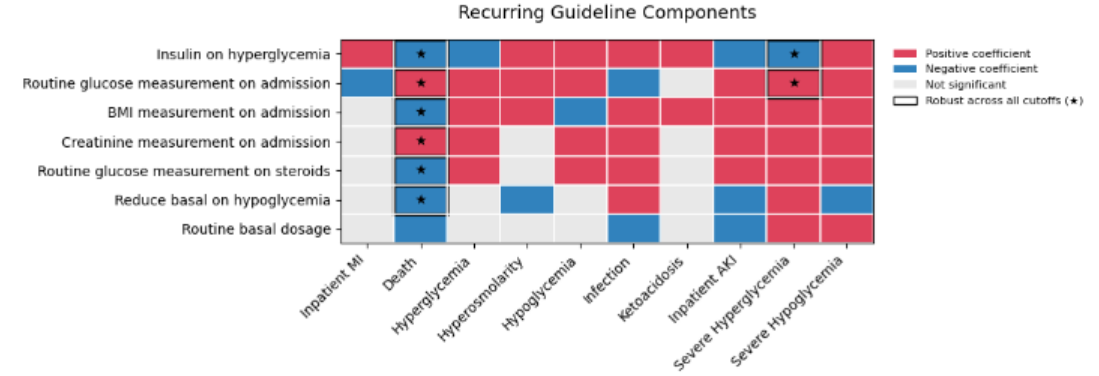
\includegraphics[width=\textwidth]{figures/recurring_guideline_components.png}
\caption{Recurring guideline-adherence components identified by the
bias-reduced regression models across clinical outcomes. Rows correspond to
guideline recommendations and columns to clinical outcomes. Colored cells
indicate statistically significant associations after false discovery rate
correction (red, positive coefficient; blue, negative coefficient). Stars
denote associations that remained significant with a consistent direction
across all three observation-window definitions (24, 48, and 72 hours). Blank
cells indicate no statistically significant association.}
\label{fig:recurring-guidelines}
\noindent\textit{Alt text:} Heatmap matrix showing recurring guideline
adherence components across ten clinical complications with direction of
association.
\end{figure}

\section{Discussion}
\label{sec:discussion}

\subsection{Principal findings}

Adherence to the national inpatient hyperglycemia recommendations improved
after their introduction, and higher adherence was consistently associated with
lower mortality and reduced hyperglycemic complications. Adherence was not
uniform: near-universal implementation was observed for several admission and
medication-management actions, whereas the largest gaps were concentrated in
insulin management. This pattern separates recommendations satisfied by a single
discrete action, such as ordering a laboratory test or discontinuing a
medication on admission, from those requiring repeated insulin decisions
across the hospitalization. The improvement was significant but modest, its $P$
value reflecting the number of admissions rather than the size of the effect,
and it was accompanied by substantial inter-hospital heterogeneity that the data
do not explain.

The clearest outcome signal was for 30-day mortality. The propensity-weighted
estimate is primary, being the only one whose exposure window---a fixed
early-admission period---is guaranteed to precede the outcome. Two descriptive
estimates agree in direction: whole-admission adherence adjusted for baseline
characteristics, and a graded fall in mortality across the adherence range. A
graded association is harder to explain by a simple difference in case mix,
though it shares the whole-admission timing concern noted below. Because the
three use different exposure definitions, they corroborate direction rather
than magnitude.

The glycemic findings show a favorable risk profile. Greater adherence bought a
large reduction in hyperglycemic burden---roughly ninefold larger on the
log-odds scale than the accompanying rise in hypoglycemia---at the cost of a
small increase in mild hypoglycemia and no detectable increase in severe
hypoglycemia, which is the balance the recommendations are intended to strike.
The same asymmetry appears at component level, where insulin following
hyperglycemia tracked lower severe hyperglycemia alongside more hypoglycemia.
Since nonsignificance is not evidence of absence, the severe-hypoglycemia
result shows no signal of harm at this sample size rather than establishing
none exists.

Adherence features ranked among the strongest retained predictors alongside
established clinical variables---the practical requirement for treating them
as monitorable quality targets. These findings have no direct precedent: the
position paper was issued in 2023, and no prior study has measured adherence
to it at this scale.

\subsection{Implications}

The most actionable pattern in these results is a convergence. The
recommendations showing the largest implementation gaps---insulin following
hyperglycemia, and the frequency and dose components of routine basal
insulin---are also among those most consistently associated with subsequent
outcomes after balancing measured baseline characteristics. The components
where practice departs most from the guideline are therefore not peripheral
ones, and this identifies them as natural targets for decision support: they
are repeated insulin decisions distributed across a hospitalization,
precisely the kind of task where a prompt at the point of care can plausibly
help, and unlike the admission recommendations they are not already at
ceiling.

This should not be read as an attribution of fault. A low adherence score
records that the action expected by the guideline is absent from the record,
not that the decision was wrong. Ward-level judgment---a patient not eating, an
imminent procedure, a deliberate decision to tolerate higher glucose in a frail
patient---is frequently the correct reason for a departure, and none of it is
recoverable from records collected for clinical rather than research purposes.
The measure is a population-level statistic, as is the inter-hospital variation
reported here. What the work offers is a
measurement instrument---an automated, component-level and transferable way to
ask which of a guideline's recommendations were followed and which track
outcomes---rather than a decision-support system.

Nothing restricts the approach to recommendations a guideline already contains.
Because each is declared externally as a pattern rather than implemented in
analysis code, a practice merely suspected to matter costs no more to evaluate
than the patterns scored here. That inverts the question: one could ask which
candidate practices earn a place in a guideline, and---more
uncomfortably---which current recommendations do not track outcomes at all.
Such candidates would be hypotheses for prospective evaluation, and a wide
search would need more conservative multiplicity correction than applied
here.

\subsection{Limitations}

The design is observational, and none of the estimates should be read as causal
effects. Residual confounding remains throughout: weighting balances only
measured covariates, and unmeasured factors---real-time illness severity above
all, and decisions to limit or de-escalate treatment---cannot be excluded.
Direction was not uniform across outcomes, reflecting differences in indication
and applicability.

The mortality analyses divide by exposure definition. The component-level and
propensity-weighted models score adherence over a fixed early-admission window,
so exposure strictly precedes outcome. The adjusted estimate instead averages
adherence over the whole admission and is descriptive: because 30-day mortality
is predominantly an end-of-admission event, and guideline-concordant management
is frequently de-escalated in patients on a deteriorating trajectory, that
average incorporates the period immediately preceding death, where adherence
may reflect the course of care rather than determine it. Dichotomizing
adherence at the median, as the weighting requires, discards dose-response
information and costs power.

Adherence and outcomes were ascertained during the same hospitalization, and
detecting glycemic events depends on glucose being measured; routine glucose
monitoring was therefore excluded from the glycemic models, though residual
detection effects may remain for other monitoring recommendations. The
pre--post comparison is uncontrolled, so secular trends in inpatient care
cannot be separated from the implementation itself, and the non-mortality
models do not account for the competing risk of death, which biases those
endpoints conservatively. The findings come from adult inpatients in Israeli
general hospitals under a single national guideline, so the adherence levels
observed and the components that proved most consequential may differ
elsewhere. Finally, the data are assembled from hospital admissions rather than
from a longitudinal record, so chronic diagnoses managed in the community may
be incompletely captured; ascertaining eligibility and glycemic outcomes from
glucose measurements rather than diagnosis codes limits the consequences, but
the comorbidity score and the proportion of hyperglycemic admissions carrying a
documented diagnosis are both likely understated.

\section{Conclusion}
\label{sec:conclusion}

Adherence to a national inpatient hyperglycemia guideline can be measured
automatically, at the level of its individual recommendations, across an entire
hospital network. Applying that measurement to 48,354 admissions in six Israeli
general hospitals shows that adherence improved after the guideline was issued,
that the improvement was modest and unevenly distributed across both
recommendations and centers, and that adherence is associated with lower 30-day
mortality and a lower burden of hyperglycemic complications once measured
baseline differences are balanced. The recommendations least well implemented
are largely the same ones whose adherence tracks subsequent outcomes: the
repeated insulin decisions distributed across a hospitalization,
rather than the single discrete actions taken on admission. That convergence,
together with the favorable shift in glycemic risk, is the evidence a guideline
needs to justify implementing it more completely. These are associations rather
than treatment effects, and they describe how a guideline was adopted rather
than how well any clinician practised. What the work establishes is that the
question is now answerable of an entire health system's records rather than of
a sample small enough to review by hand.


% ---------------------------------------------------------------------
% End matter
% ---------------------------------------------------------------------
% =====================================================================
% JAMIA end matter. Oxford orders these sections: Author Contributions,
% Supplementary Material, Acknowledgments, Funding, Conflicts of
% Interest, Data Availability.
% =====================================================================

\section*{Author Contributions}
\textbf{Shahar Oded:} conceptualization, methodology, software, validation,
formal analysis, data curation, visualization, writing---original draft.
\textbf{Yuval Shahar:} conceptualization, methodology, supervision, funding
acquisition, writing---review and editing.
\textbf{Erez Shalom:} resources, project administration, writing---review and
editing.
\textbf{Amir Bashkin}, \textbf{Leonard Saig}, \textbf{Dror Cantrell},
\textbf{Irit Wirsansky}, \textbf{Muhamad Badarne}, and \textbf{Irena Barash:}
investigation, resources, writing---review and editing.
\textbf{Avivit Cahn:} conceptualization, investigation, writing---review and
editing.
\textbf{Irit Hochberg:} conceptualization, methodology, validation,
resources, supervision, writing---review and editing.

\section*{Supplementary Material}
Supplementary material is available at \emph{Journal of the American Medical
Informatics Association} online. Appendix~S1 details data preparation, the
concept index, the modified Charlson comorbidity index, threshold
acquisition, score aggregation, and software. Appendix~S2 gives the
operational definitions of all ten complications. Appendix~S3 gives the
operational definitions of the fourteen assessed guideline recommendations.
Table~S2 summarizes the bias-reduced regression models. The curated concept
indices are supplied as a separate data file.

\section*{Acknowledgments}
This study would not have been possible without the Kineret project team, who
built and maintain the harmonized multicenter data warehouse on which it
rests. Transforming the records of a national hospital network into a common
data model, and sustaining the infrastructure and governance that make it
usable for research, represents a substantial body of work in its own right;
the authors are grateful for that effort and for the team's support in
accessing the data and extracting the study cohort. The authors also thank
the Helsinki committee coordinators at the participating centers for their
assistance throughout the approval process.

\section*{Funding}
\TODO{Funding statement outstanding --- see open task 1 on the title page.}

\section*{Conflicts of Interest}
Several of the authors contributed to the national position paper whose
implementation is assessed in this study. The authors declare no competing
financial interests or personal relationships that could have appeared to
influence the work reported in this paper.

\section*{Data Availability}
The abstraction engine, the knowledge base of temporal-abstraction and
quality-assessment definitions, and the analysis notebooks are publicly
available in the Mediator repository \citep{mediator-github}, and the
extraction and cohort-construction pipeline in a companion repository
\citep{kineret-etl-github}. The curated concept indices mapping the source
vocabulary onto the concepts named in the knowledge base are provided as
supplementary material.

All processing and analysis were performed inside a closed hospital computing
environment. The code released here is a replica of that pipeline; no source
data, intermediate datasets, or unaggregated outputs leave that environment,
and the results reported in this paper are exported aggregate statistics. The
underlying patient-level electronic health record data cannot be shared, as
it comprises identifiable clinical records governed by the approvals under
which it was obtained.

\section*{Ethics Approval}
The study was approved by the institutional Helsinki committee of each
participating center under a common protocol (NHR-0152-23): Galilee Medical
Center (NHR-0152-23), Hillel Yaffe Medical Center (HYMC-0074-24), Shamir
Medical Center (ASF-0117-24), Tzafon Medical Center (POR-0047-24), Barzilai
University Medical Center (BRZ-0059-24), and Bnai Zion Medical Center
(BNZ-0067-24). Recruitment was approved for up to 30,000 participants across
all centers combined. A full waiver of informed consent was granted, since
the study extracts records from a de-identified repository with no patient
contact.


\bibliographystyle{unsrtnat}
\bibliography{references}

\end{document}
